\subsection{Sensoren in der Testkammer}\label{sec:Sensoren in der Testkammer}
Die verschiedenen Sensoren werden in der Testkammer platziert, damit einen Vergleich zwischen den Sensorwerten in der Kammer und auf dem CubeSat dargestellt werden kann. Dieser Vergleicht ist eine Überprüfung, ob alle Sensoren auf dem CubeSat noch funktionieren und richtige Werte ausgeben. Bei den verwendeten Sensoren musste darauf geachtet werden, dass sie bei einer Temperatur von 0°C bis 30°C betrieben werden können.
\begin{figure}[H]
	\centering
	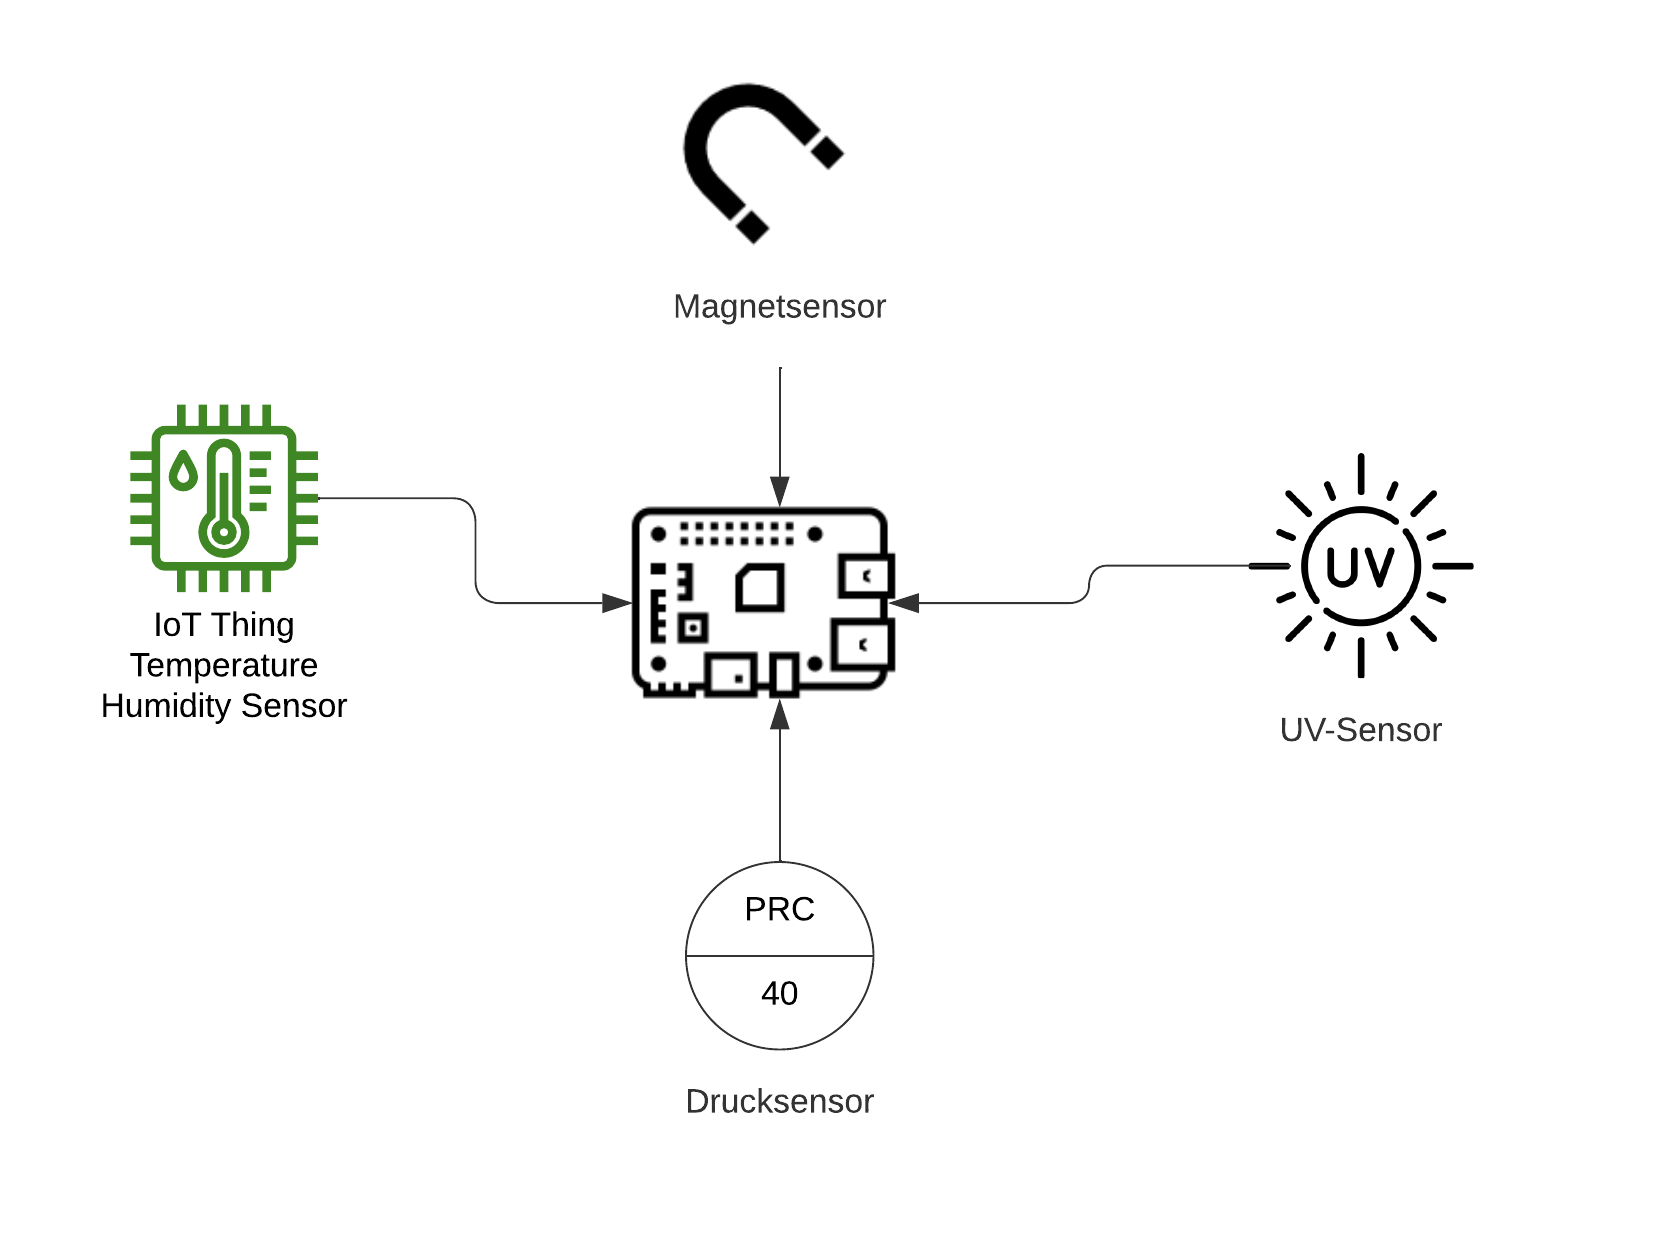
\includegraphics[scale=0.3]{image/blocksensor.png}
	\caption{Blockschaltbild Sensoren}
\end{figure}

\newpage
\subsubsection{Temperatursensor}\label{sec:Temperatursensor}
In der Testkammer befinden sich zwei Temperatursensoren mit integriertem Feuchtigkeitssensoren. Diese messen die Temperatur sowie die Feuchtigkeit in der Kammer. Dadurch können die Sensorwerte der Kammer und des CubeSat verglichen werden.\\
\vspace{3mm}
Für diese Anwendung wird der Temperatursensor \textbf{AM2302} \autocite{AM2302} verwendet. Der Anschluss an den \raspi erfolgt durch die PCB. Der Sensor wird mit 3 Pins an die PCB angeschlossen.\\
\vspace{3mm}
\begin{table}[H]
    \centering
    \begin{tabular}{ | c | c | } 
  \hline
   VDD & 5 Volt\\ 
  \hline
   GND & Ground\\ 
  \hline
   Data & GPIO7 und GPIO8\\ 
  \hline
\end{tabular}
    \caption{Pinbelegung Temperatursensor}
\end{table}
Um beide Sensoren in der Testkammer zu montieren, wurde ein Gehäuse in SolidWorks entworfen. Danach wurden die Teile mit dem 3D-Drucker ausgedruckt.\\
\vspace{2mm}
\begin{figure}[H]
\centering
\includegraphics[scale=0.6]{image/Gehäusetemp.png}
\caption{Gehäuse Temperatursensor}
\end{figure}
\newpage
Um den Temperatursensor zu verwenden, wird eine Bibliothek benötigt. Die Bibliothek wird von Adafruit bereitgestellt. Um diese zu installieren wird folgender Befehl auf dem \raspi ausgeführt:\\
\begin{verbatim}
pip3 install adafruit-circuitpython-dht
\end{verbatim}
Durch die Bibliothek\autocite{Adafruit_DHT} wird das Auslesen des Sensors vereinfacht. Mit wenigen Befehlen kann der Sensor die Temperatur und die Feuchtigkeit messen.\\
\vspace{3mm}
\begin{figure}[H]
    \centering
    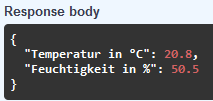
\includegraphics[scale=1.5]{image/Tempausgabe.png}
    \caption{Temperatursensorausgabe}
    \label{fig:enter-label}
\end{figure}
Die Messung mit dem Temperatursensor wurden in einem normalen Zimmer mit Raumtemperatur durchgeführt. Die ermittelten Daten für Temperatur und Feuchtigkeit werden in der oberen Abbildung abgebildet.\\
\vspace{3mm}
Die Programmierung für das Testprogramm befindet sich im Kapitel \ref{sec:Testprogramm Temp}, und der Programm Abschnitt für die API im Kapitel \ref{sec:API-Temp}





\subsubsection{UV-Sensor}
Der CubeSat besitzt einen UV-Sensor, aus diesem Grund wurde auch in die Testkammer einer eingebaut. Es wurde der UV-Sensor LTR390\autocite{LTR390} verwendet. Dieser verfügt über einen integrierten ADC, somit muss kein Analog-Digital-Wandler dazwischengeschaltet werden und kann direkt über I2C an den \raspi angeschlossen werden.\\
\vspace{5mm}
\begin{table}[H]
    \centering
    \begin{tabular}{ | c | c | } 
  \hline
   VCC & 5 Volt\\ 
  \hline
   GND & Ground\\ 
  \hline
   SDA & GPIO3 \\ 
  \hline
   SCL & GPIO5 \\ 
  \hline
   INT & Interruptausgang \\ 
  \hline
\end{tabular}
    \caption{Pinbelegung UV-Sensor}
\end{table}
\begin{figwindow}[0,r,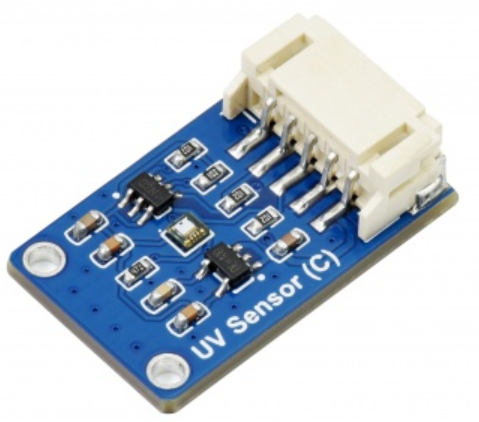
\includegraphics[scale=0.5]{image/UVsensor.png},{UV-Sensor}]
Das Licht der UV-Lampe\ref{sec:UV-Lampe} hat eine Wellenlänge von 385nm bis 400nm. Daher muss der UV-Sensor auch für diesen Bereich ausgelegt sein. Der Messbereich des LTR390 ist zwischen 200nm und 400nm. Der Sensor misst das Umgebungslicht und den UV-Index. Das Umgebungslicht wird in Lux angegeben. Ein niedriger Lux-Wert bedeutet das der Sensor sich in einer dunklen Umgebung befindet. Ein hoher Wert bedeutet eine helle Umgebung. Der UV-Index wird in verschiedene Kategorien eingeteilt.
\end{figwindow}
\vspace{2mm}
\begin{table}[h]
    \centering
    \begin{tabular}{ | c | c | } 
  \hline
   UV-Index & Kategorie\\ 
  \hline
   0-2 & Niedrig\\ 
  \hline
   3-5 & Mäßig \\ 
  \hline
   6-7 & Hoch \\ 
  \hline
   8-10 & sehr Hoch \\ 
  \hline
   11+ & Extrem \\ 
  \hline
\end{tabular}
    \caption{UV-Index}
\end{table}

\begin{figure}[H]
    \centering
    \begin{subfigure}[b]{0.45\textwidth}
        \centering
        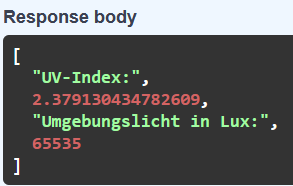
\includegraphics[width=\textwidth]{image/UVsensor hell.png}
        \caption{indirektes Sonnenlicht}
        \label{fig:bild1}
    \end{subfigure}
    \hfill
    \begin{subfigure}[b]{0.45\textwidth}
        \centering
        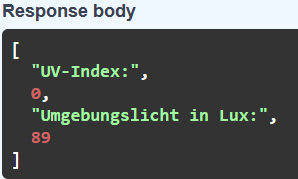
\includegraphics[width=\textwidth]{image/uvsensor dunkel.png}
        \caption{kein Sonnenlicht}
        \label{fig:bild2}
    \end{subfigure}
    \caption{Messungen mit UV-Sensor}
    \label{fig:zwei_bilder}
\end{figure}
Die Messungen der oberen zwei Abbildungen wurden in einem Zimmer durchgeführt. Der Sensor in Abbildung (a) wurde für die Messung dem Sonnenlicht durch ein Fenster ausgesetzt. Aus diesem Grund ist der UV-Index eher niedrig. Der LTR390 kann Umgebungslicht von 0 Lux bis zu 65535 Lux messen. In Abbildung (a) ist zu erkennen, dass der maximale Wert bei der Messung des Umgebungslichtes erreicht wurde. Daraus kann geschlussfolgert werden, dass sich der Sensor in einer hellen Umgebung befunden hat. In Abbildung (b) wurde der Sensor vom Sonnenlicht entfernt, somit haben keine UV-Strahlen den Sensor getroffe. Dies kann auch am gemessenen UV-Index erkennt werden. Es wurde ein Umgebungslicht von 89 Lux gemessen. Der UV-Sensor war also in einer eher dunklen Umgebung.\\
Für den LTR390 UV-Sensor wird die folgende Bibliothek\autocite{LTR390} verwendet:
\begin{verbatim}
pip install adafruit-circuitpython-ltr390
\end{verbatim}
\vspace{3mm}
Das Testprogramm für den UV-Sensor ist im Kapitel \ref{sec:Testprogramm UV-Sensor} und der Codeabschnitt für die API im Kapitel \ref{API-UVS}
\subsubsection{Magnetsensor}\label{sec: Magnetsensor}
Der Magnetsensor misst das Magnetfeld in seiner Umgebung. Der KY-024 Linearer, magnetischer Hall-Sensor\autocite{KY-024}, ist für den Dauerbetrieb geeignet und ist in einem Temperaturintervall von -150°C bis 150°C stabil. \\
\vspace{3mm}
\begin{figure}[H]
    \centering
    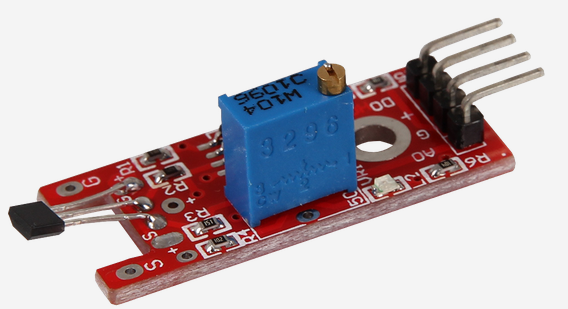
\includegraphics[scale=0.8]{image/magnetsensir.png}
    \caption{KY-024 Magnetsensor}
    \label{fig:enter-label}
\end{figure}
\vspace{3mm}
Der Sensor besitzt zwei LEDs. 
\begin{itemize}
    \item LED 1: zeigt an, ob der Sensor mit Strom versorgt wird.
    \item LED 2: zeigt an, ob der Sensor ein Magnetfeld erkannt hat.
\end{itemize}
\vspace{3mm}
Durch ein Drehpotentiometer kann die Empfindlichkeit des Sensors eingestellt werden. Über den digitalen Ausgang des Sensors wird ein Signal ausgegeben, sobald ein Magnetfeld erkannt wird.\\
\newpage
Der KY-024 ist ein analoger Sensor. Da der \raspi keinen integrierten ADC besitzt, muss einer gekauft werden, damit der Sensor über den \raspi angesteuert und gelesen werden kann. Als ADC eignet sich hierfür der 16-Bit ADC KY-053\autocite{KY-053}. \\
\vspace{2mm}
\textbf{Zusammenschaltung von \raspi, Magnetsensor und ADC}
\begin{figure}[H]
    \centering
    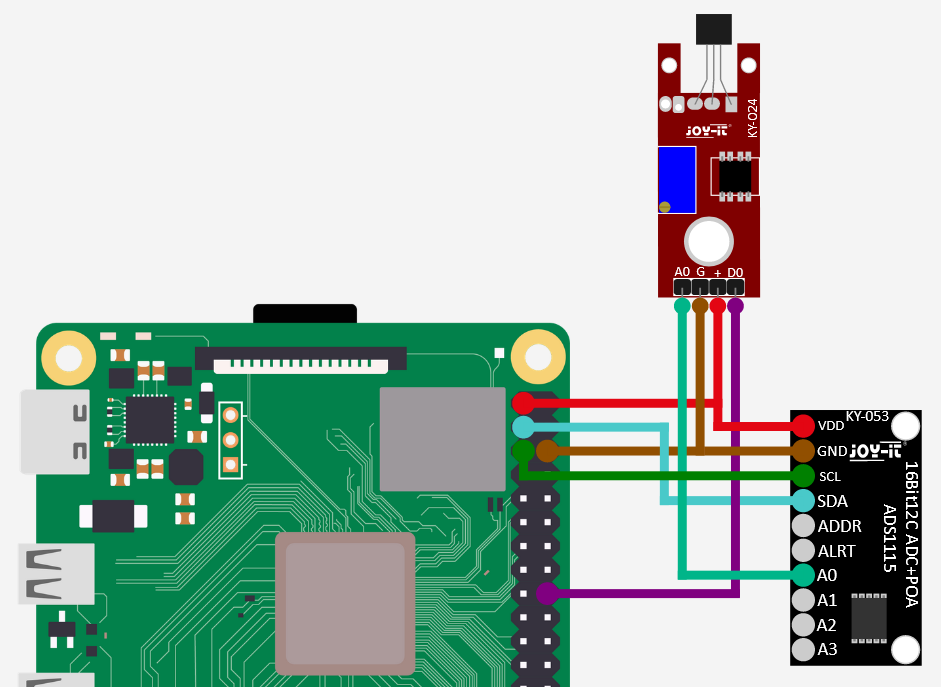
\includegraphics[scale=0.6]{image/zusammenmanet.png}
    \caption{Zusammenschaltung Magnetsensor\autocite{Zusammenschaltungmagnet}}
    \label{fig:enter-label}
\end{figure}
\subsubsection{Drucksensor}
In der Teststation gibt es eine Vorrichtung, um ein Vakuum zu erzeugen. Durch dieses Vakuum kann der integrierte barometrischer Drucksensor auf dem CubeSat getestet werden. Der Drucksensor in der Kammer wird dazu verwendet, einen Vergleich zwischen Testkammer und Satellit herzustellen.\\
\vspace{3mm}
Es wurde der Drucksensor BMP180\autocite{BMP180} verwendet. Er befindet sich in der Testkammer, hat jedoch keinen fixen Platz. Der Sensor kann je nachdem, ob ein Vakuum erzeugt wird oder nicht, platziert werden. Der BMP180 hat 4 Pins die über die PCB angeschlossen und mit dem \raspi verbunden. werden.\\
\vspace{3mm}
\begin{table}[h]
    \centering
    \begin{tabular}{ | c | c | } 
  \hline
   Vin & 5 Volt\\ 
  \hline
   GND & Ground\\ 
  \hline
   SDA & GPIO3 \\ 
  \hline
   SCL & GPIO5 \\ 
  \hline
\end{tabular}
    \caption{Pinbelegung Drucksensor}
\end{table}
\vspace{3mm}
Um den Sensor verwenden zu können, muss auch hier eine Bibliothek heruntergeladen werden. Diese wird von Adafruit bereitgestellt. Mit folgendem Befehl kann die Bibliothek\autocite{BMP180bib} heruntergeladen werden.
\begin{verbatim}
pip install circuitpython-bmp180
\end{verbatim}
Die Suche nach einer geeigneten Bibliothek war nicht einfach, da die meisten Repository archiviert wurden. In einigen Dokumenten wird auch angegeben, dass der Drucksensor BMP180 gar nicht mehr hergestellt wird.\\
\vspace{3mm}
\begin{figure}[H]
    \centering
    \begin{subfigure}[b]{0.7\textwidth}
        \centering
        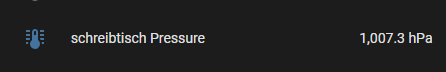
\includegraphics[width=\textwidth]{image/druckvergleich.png}
        \caption{Messung über Wetterstation}
        \label{fig:bild1}
    \end{subfigure}
    \hfill
    \begin{subfigure}[b]{0.5\textwidth}
        \centering
        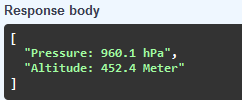
\includegraphics[width=\textwidth]{image/druckausgabe.png}
        \caption{Messung mit Drucksensor}
        \label{fig:bild2}
    \end{subfigure}
    \caption{Druckmessungen}
    \label{fig:zwei_bilder}
\end{figure}
Die oben angeführten Druckmessungen, wurden beide in Wolfurt durchgeführt. Der Druck in Abbildung (a), wurde mit einer Netatmo Wetterstation\autocite{Netatmo} gemessen. In Abbildung (b), wurde der BMP180 Drucksensor verwendet, um den Druck zu ermitteln. Die Werte stimmen einigermaßen überein. Auch die Meereshöhe kann mit dem BMP180 angezeigt werden. Wolfurt liegt auf einer Meereshöhe von 434 m. Der Sensor zeigt eine Meereshöhe von 452 Metern an. Da dieser Wert nicht genau mit dem tatsächlichen Wert über einstimmt, kann eine Kalibrierung durchgeführt werden. Dies erfolgt durch eine Anpassung an der Berechnung im Code.\\
\vspace{3mm}
Der Codeabschnitt für das Testprogramm befindet sich im Kapitel  \ref{sec:Testprogramm Drucksensor}. Das Programm für die API ist im Kapitel \ref{sec:API-Druck}.